\documentclass[12pt,a4paper]{article}
\usepackage[utf8]{inputenc}
\usepackage[T1]{fontenc}
\usepackage{amsmath}
\usepackage{amsfonts}
\usepackage{amssymb}
\usepackage{lipsum}
\usepackage{textcomp}

\usepackage{makecell} % linebreak dans une cellule
\usepackage{multicol} % twocols localement
\usepackage{vwcol} % idem mais avec largeur variable
\usepackage{color, colortbl} % colorer les tableaux
\usepackage{enumitem} % utiliser des lettres pour énumérer
\usepackage{wrapfig} % insérer des images dans dutexte
\usepackage{dashundergaps} % transformer du texte en ________
\usepackage{MnSymbol,wasysym} % smileys
\usepackage{ifthen}
\usepackage{soul} % teste barré \st

% --- geometry ---
\usepackage{geometry}
\geometry{legalpaper, margin=2cm}
% ---

% --- xcolor ---
\usepackage{xcolor}
\definecolor{lightgray}{gray}{0.9}
% ---

% --- tcolorboxes ---
\usepackage[most]{tcolorbox}
\newtcolorbox{definition}[2][]{%
  attach boxed title to top left
               = {yshift=-8pt},
  colback      = white,
  colframe     = gray,
  fonttitle    = \bfseries,
  colbacktitle = gray,
  title        = #2,#1,
  enhanced,
}
% ---


\renewcommand{\baselinestretch}{1.15} % augmenter l'interligne

\dashundergapssetup{
	teacher-gap-format=underline,
	gap-widen
}



\author{Paul Clavier}
\title{Chapitre 5 - Droites parallèles et perpendiculaires}

\begin{document}

% --- Section & subsection renum ---
\renewcommand\thesection{\Roman{section}}
\renewcommand\thesubsection{\arabic{subsection}}
% ---

% --- Selection manuelle de la version ---
\def\isprof{true}
% ---

% --- Selection automatique de la version ---
\ifdefined\isprof
	\TeacherModeOn
\fi

% ---



\begin{center}
	\fbox{\parbox{\dimexpr\linewidth-2\fboxsep-2\fboxrule\relax}{\centering\huge Chapitre 5 - Droites parallèles et perpendiculaires}}
\end{center}

\section{Droites perpendiculaires}

\begin{definition}{Définition}
Deux droites sont \gap*{perpendiculaires} si elles sont \gap*{sécantes} en formant un \gap*{angle droit}.
\end{definition}

\textbf{Exemple}: \\
\begin{minipage}{0.5\textwidth}
\ifdefined\isprof
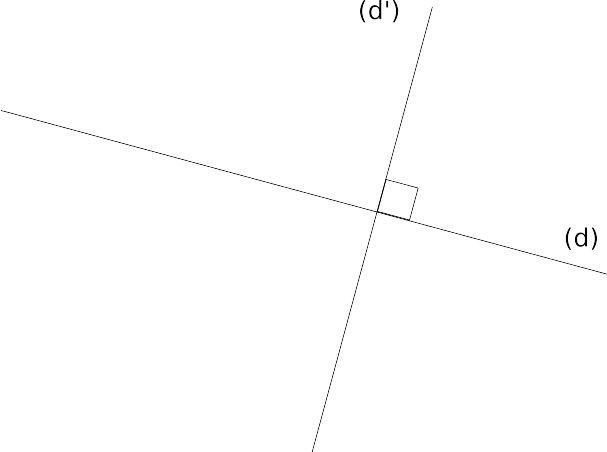
\includegraphics[scale=0.4]{img/perpendiculaires.png} 
\else
\phantom{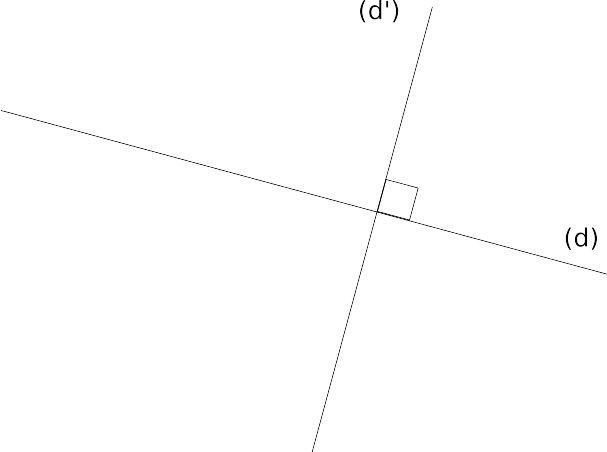
\includegraphics[scale=0.5]{img/perpendiculaires.png}}
\fi
\end{minipage}
\begin{minipage}{0.4\textwidth}
Les droites $(d)$ et $(d')$ sont perpendiculaires. On note $(d) \perp (d')$.
\end{minipage}\\

\textbf{Exemple 2}: Construire la droite perpendiculaire à $(d)$ passant pas le point $M$.

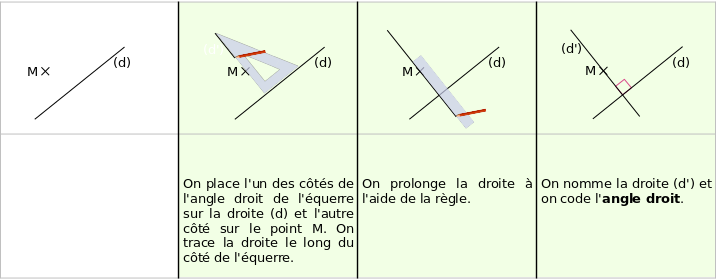
\includegraphics[scale=1]{img/construction-perpendiculaires.png} 

\section{Droites parallèles}

\begin{definition}{Définition}
Deux droites sont \gap*{parallèles} si elles ne sont pas \gap*{sécantes}.
\end{definition}

\textbf{Remarque}:
\begin{itemize}
\item soit deux droites parallèles sont confondues
\item soit elles n'ont aucun point en commun
\end{itemize}

\textbf{Exemple 2}: Construire la droite parallèle à $(d)$ passant par le point $M$.

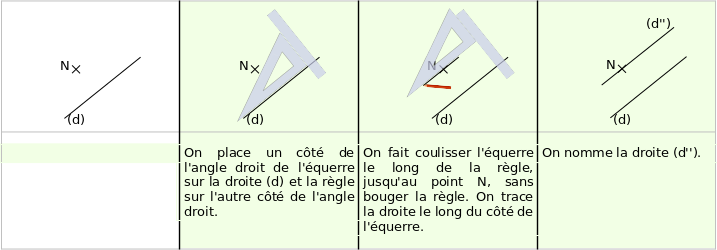
\includegraphics[scale=1]{img/construction-parallele.png} 

\section{Position relative de deux droites}

\begin{minipage}{0.35\textwidth}
\begin{definition}{Propriété 1}
Deux droites sont soit sécantes, soit parallèles.
\end{definition}
\begin{definition}{Propriété 2}
Deux droites sécantes sont soit perpendiculaires, soit non perpendiculaires.
\end{definition}
\end{minipage}
\begin{minipage}{0.7\textwidth}
\textbf{Remarque}: On peut résumer ceci dans un organigramme.
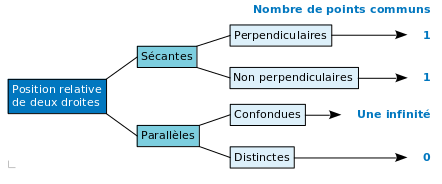
\includegraphics[scale=1]{img/position-relative.png} 
\end{minipage}

\section{Propriété des droites parallèles et perpendiculaires}

\begin{definition}{Propriété 1}
Si deux droites sont perpendiculaires à une troisième droite, alors ces deux droites sont parallèles.
\end{definition}
\begin{minipage}{0.7\textwidth}
\textbf{Exemple}: On sait que $(d)\perp(d')$ et que $(d')\perp(d'')$ donc $(d)\parallel (d'')$
\end{minipage}
\begin{minipage}{0.3\textwidth}
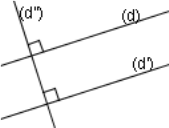
\includegraphics[scale=1]{img/prop1.png} 
\end{minipage}

\begin{definition}{Propriété 2}
Si deux droites sont parallèles à une troisième droite, alors ces deux droites sont parallèles.
\end{definition}
\begin{minipage}{0.7\textwidth}
\textbf{Exemple}: On sait que $(d)\parallel(d')$ et que $(d')\parallel(d'')$ donc $(d)\parallel (d'')$
\end{minipage}
\begin{minipage}{0.3\textwidth}
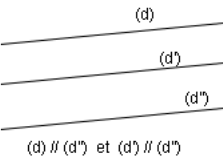
\includegraphics[scale=1]{img/prop2.png} 
\end{minipage}

\begin{definition}{Propriété 1}
Si deux droites sont parallèles alors toute droite perpendiculaire à l'une est perpendiculaire à l'autre.
\end{definition}
\begin{minipage}{0.7\textwidth}
\textbf{Exemple}: On sait que $(d)\parallel(d')$ et que $(d)\perp(d'')$ donc $(d')\perp (d'')$
\end{minipage}
\begin{minipage}{0.3\textwidth}
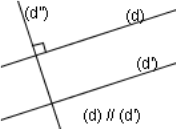
\includegraphics[scale=1]{img/prop3.png} 
\end{minipage}

\end{document}